\documentclass[11pt]{article}
\usepackage[utf8]{inputenc}
\usepackage[T1]{fontenc}
\usepackage[margin=0.85in]{geometry}
\usepackage{graphicx}
\usepackage{amssymb}
\usepackage{microtype}
\usepackage{enumitem}
\usepackage{xcolor}
\usepackage{tikz}
\usetikzlibrary{arrows.meta,positioning}
\usepackage{float}
\usepackage{multicol}
\usepackage[hidelinks]{hyperref}
\usepackage{titling}
\graphicspath{{figures/}}

\setlength{\droptitle}{-3.5em}
\setlist{nosep,leftmargin=1.3em}
\pagestyle{empty}

\title{\vspace{-1em}\textbf{\large Globally-Mapped LiDAR Navigation for a Quadruped Robot}\\[-0.2em]
\normalsize Executive Summary}
\author{}
\date{}

\begin{document}
\maketitle
\vspace{-3.5em}

\noindent\small
\textbf{Author:} Sanjit K. (research intern), Southern Methodist University \hfill
\textbf{Date:} June 22, 2026\\[2pt]
\rule{\linewidth}{0.4pt}

\vspace{2pt}
\noindent\textbf{Objective.}
Reproduce and extend the classical navigation stack of a recent IEEE study on
quadruped path planning \cite{refpaper} --- \emph{LiDAR mapping $\rightarrow$
localization $\rightarrow$ global planning $\rightarrow$ local obstacle avoidance}
--- and steer it toward our target application, autonomous \textbf{person-following}
\cite{islam2019}, where the robot tracks a moving person rather than a fixed goal.
The whole stack was built from scratch in Python (\texttt{numpy} only; no heavy
dependencies) and validated on synthetic, real automotive-LiDAR, and indoor RGB-D data.

\vspace{4pt}
\noindent\textbf{What was built.}
\begin{itemize}
  \item \textbf{2.5D terrain map} --- raw point clouds discretized into a per-cell
  height grid that keeps the steps/slopes/gaps a legged robot cares about, with a
  per-cell \textbf{Kalman filter} \cite{kalman1960,fankhauser2018} fusing repeated
  scans to reduce noise and flag low-confidence cells.
  \item \textbf{Global planner} --- Dijkstra/A$^\star$ shortest path
  \cite{dijkstra1959,hart1968} over a traversability cost grid, then geometric
  (elastic-band / TEB-style) smoothing \cite{rosmann2017}.
  \item \textbf{Local planner} --- artificial potential field (Khatib)
  \cite{khatib1986} for real-time obstacle avoidance, with a moving-goal mode for
  person-following.
  \item \textbf{Deployment path} --- a ROS\,2 / Nav2 node \cite{macenski2020} that
  publishes the map as a costmap layer; plus 2D and interactive 3D visualizations.
\end{itemize}

\begin{figure}[h]
\centering
\begin{tikzpicture}[node distance=4mm and 7mm,
  box/.style={draw,rounded corners,align=center,minimum height=7mm,inner sep=2.5pt,
    font=\scriptsize,fill=blue!4},
  impl/.style={box,fill=green!7}, ext/.style={box,fill=orange!10},
  >={Stealth[]}, every edge/.style={draw,->,semithick}]
  \node[box] (s){LiDAR / GPS / IMU};
  \node[box,right=of s](l){SLAM loc.\\\scriptsize(assumed)};
  \node[impl,right=of l](m){Kalman 2.5D\\map};
  \node[impl,right=of m](c){Cost grid};
  \node[impl,right=of c](g){Dijkstra /\\A$^\star$};
  \node[impl,below=5mm of g](t){TEB smooth};
  \node[impl,left=of t](a){APF local};
  \node[ext,left=of a](p){Moving goal\\\scriptsize(person)};
  \node[box,left=of p](ctrl){Quadruped\\control};
  \draw(s)edge(l); \draw(l)edge(m); \draw(m)edge(c); \draw(c)edge(g);
  \draw(g)edge(t); \draw(t)edge(a); \draw(p)edge(a); \draw(a)edge(ctrl);
\end{tikzpicture}
\\[-2pt]
{\scriptsize System architecture. Green = implemented; orange = person-following
extension; white = assumed input.}
\label{fig:arch}
\end{figure}

\vspace{-2pt}
\noindent\textbf{Key findings.}
\begin{enumerate}
  \item \textbf{Clean LiDAR works out of the box; noisy RGB-D does not.}
  The same code handles real KITTI \cite{geiger2013} automotive scans at default
  settings, but a single-view RGB-D floor has \mbox{$\sim$15--20\,cm} of depth
  noise per cell and needs looser tolerances. \emph{Traversability thresholds are
  sensor-specific, not universal constants.}
  \item \textbf{Multi-scan fusion needs localization.} Fusing two real LiDAR scans
  taken from different robot poses inflated obstacle cells by $\sim$80\% through
  ghosting; fusing a scan with itself did not. This empirically shows why the
  reference stack requires the SLAM/ICP \cite{besl1992} localization stage that we
  left as an assumed input.
  \item \textbf{The global planner is essential, not decorative.} Pure APF toward a
  distant goal got trapped in a local minimum 4.4\,m short; pairing it with the
  global path (APF following a moving sub-goal) reached the goal while keeping
  $\sim$0.5\,m obstacle clearance. The person-following mode tracked a walking
  target at a $\sim$0.6\,m mean gap.
\end{enumerate}

\vspace{2pt}
\noindent\textbf{Status \& next steps.}
The mapping, planning, smoothing, avoidance, person-following, Nav2 integration, and
visualization components are implemented and covered by 21 passing unit tests. The
main remaining piece is the \textbf{localization} stage (ICP / LiDAR-inertial
odometry) to supply robot poses for true multi-scan fusion, followed by the
person-following \textbf{perception front-end} (camera-based detection and tracking)
and on-robot testing through the Nav2 interface. A full technical report with
methods, equations, and all figures accompanies this summary.

\begin{figure}[H]
\centering
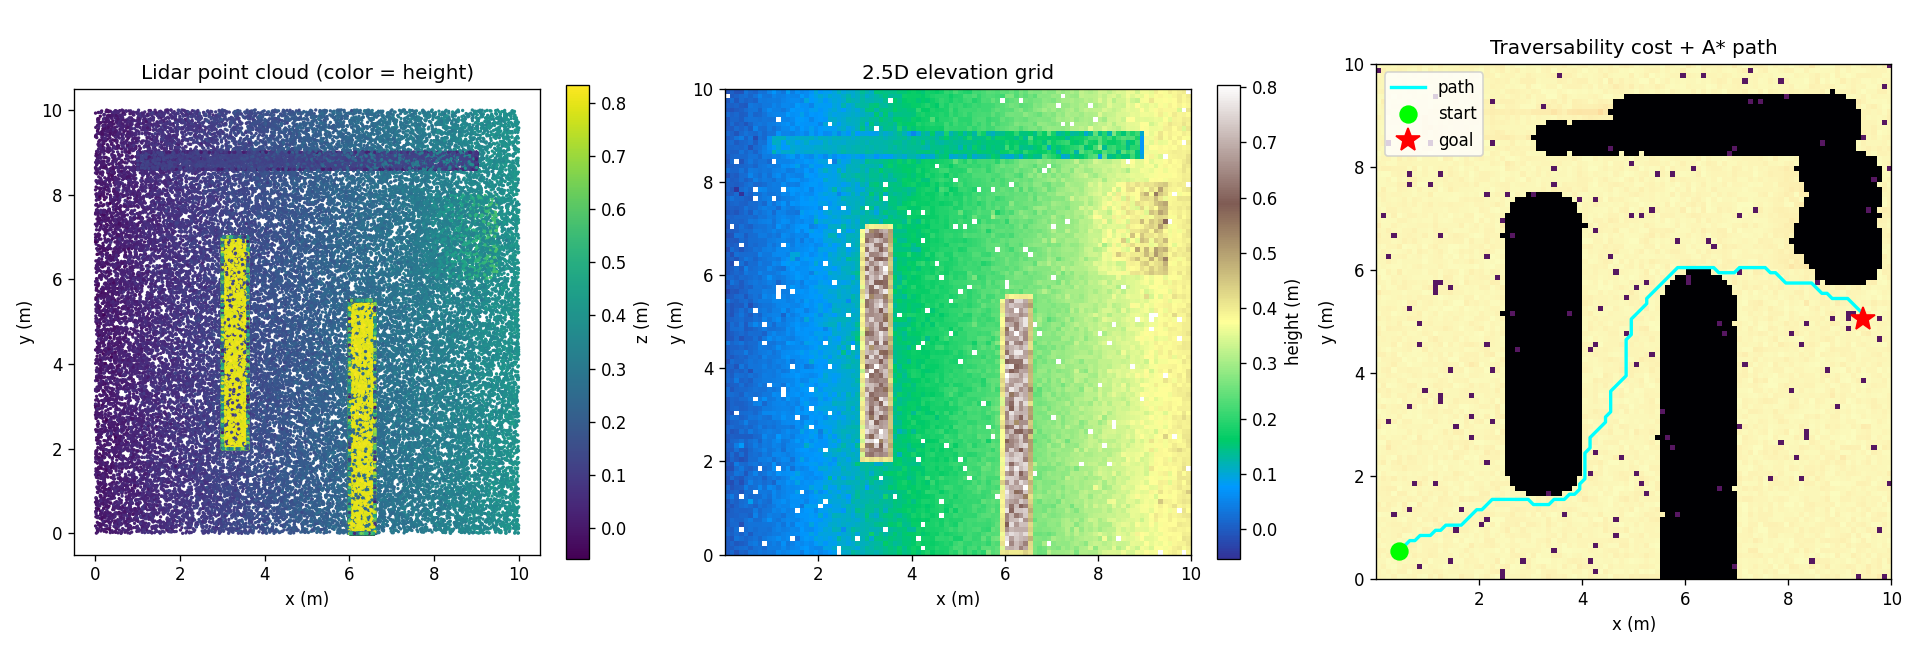
\includegraphics[width=0.9\linewidth]{out.png}\\[2pt]
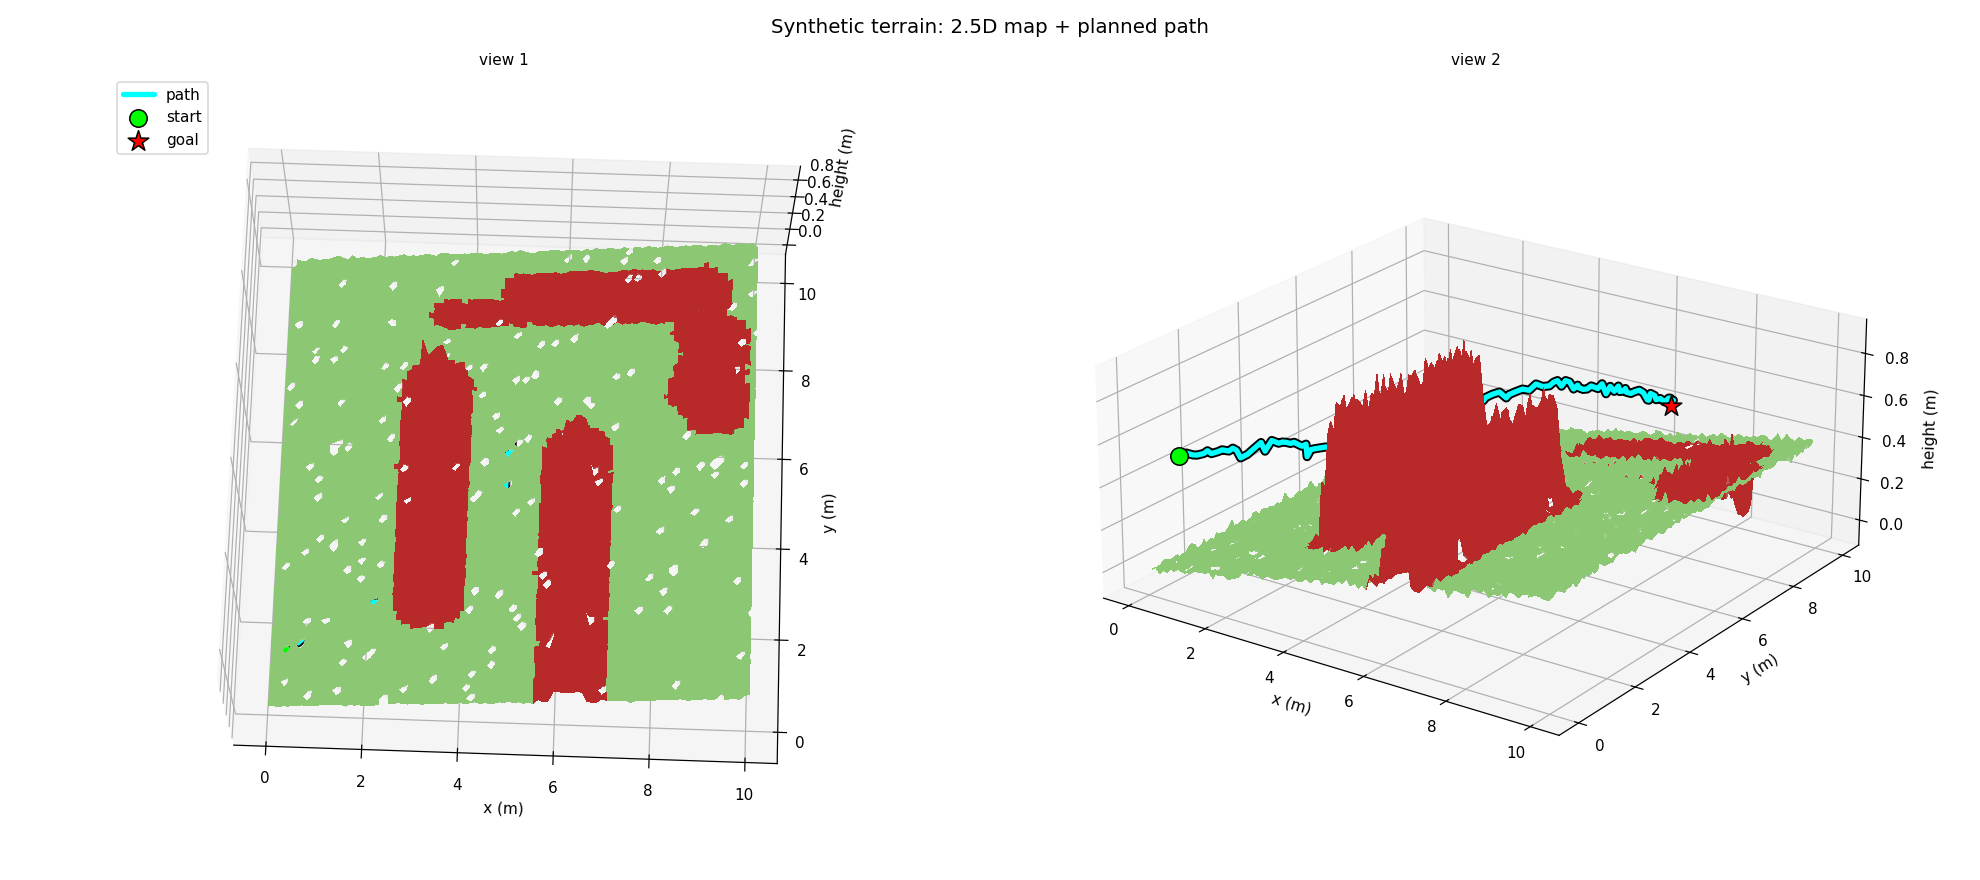
\includegraphics[width=0.52\linewidth]{out_3d.png}
\\[1pt]
{\scriptsize Example results. \textbf{Top:} point cloud $\rightarrow$ 2.5D
elevation grid $\rightarrow$ cost grid with the planned A$^\star$ path.
\textbf{Bottom:} the same map in 3D, path draped over the terrain
(green = traversable, red = obstacle).}
\label{fig:results}
\end{figure}

\vspace{3pt}
{\scriptsize
\renewcommand{\section}[2]{\noindent\textbf{References.}\par\nobreak}
\begin{multicols}{2}
\bibliographystyle{ieeetr}
\bibliography{references}
\end{multicols}
}

\end{document}
